\documentclass{jmlr} % W&CP article

\usepackage{booktabs}

\usepackage[load-configurations=version-1]{siunitx} % newer version
 % The following command is just for this sample document:
\newcommand{\cs}[1]{\texttt{\char`\\#1}}% 
\theorembodyfont{\upshape}
\theoremheaderfont{\scshape}
\theorempostheader{:}
\theoremsep{\newline}
\newtheorem*{note}{Note}
\jmlrproceedings{HSE ML PROJECT}{ML project GPVAE}

\title[GP-VAE for Latent Dynamics in 3D]{GPVAE for Latent Dynamics from Pixels in 3 Dimension}
\author{\Name{Bhupendra Dubey}\\
  \addr Higher School of Economics}
\begin{document}
\maketitle
\section{Introduction}
\label{sec:intro}
 In this project we consider learning problem of latent state of pixels from a video containing a moving object in three dimension. We extend the work done by \citep{pearce19}. In the original work the Gaussian
Process Prior Variational Autoencoder (GPP-VAE) was used to learn intermediate latent representations from features (input) to images (output). In the original work two-dimensional data was used to learn the latent representation. Here we try to learn latent representation of pixels in three dimension. We use Gaussian Process Prior to a standard Variational Autoencoder to learn the latent dynamics.

\section{Motivation}
For a given a dataset of images and each image has a corresponding feature vector,
e.g. images of faces and features are pose angle, lighting intensity etc. We will try to use GPPVAE to learn these intermediate latent representation from these features to the output relationship.


\section{The Gaussian Process Prior for VAE}

\subsection{Generative model}
In this setting we consider videos of single moving object. Each video consists of a set of $T$ 3D-images: $v_1, ..., v_T$ $\in$ $[0, 1]^{16X16X16}$ which are binary
matrices and the corresponding feature of an image is its time stamp $t$. The intermediate
state we aim to learn is an interpretable 3D latent time-series of $x_{1:T}$ , $y_{1:T}$ , $z_{1:T}$ coordindates for
the object for each frame. We have no ground truth data of object position hence this is
unsupervised. We place a Gaussian process prior over time on the functions $x, y, z : [1, T] \to \mathbb{R}$. 
A Gaussian process may be viewed as a more general linear Gaussian state space model,
this has the benefit of being more flexible, and smoothing (aggregating information across
all time) is performed by default.  $\mathcal{B}(v_t|p_{\theta}(x_t,y_t,z_t))$ is a product of 16X16X16 independent Bernoulli distributions over pixels
parameterised by a neural network  $p_{\theta}(x_t,y_t,z_t)$ (parameters $\theta$) which is probability of a pixel to be 1. 

The generative model is given by
$$\mathbb{P}[v_{1:T}, x_{1:T}, y_{1:T}, z_{1:T}] = \prod_{t=1}^{T}\mathbb{P}[v_t|x_t,y_t,z_t]\mathbb{P}[x_{1:T}, y_{1:T}, z_{1:T}]$$
$$= \prod_{t=1}^{T}\mathcal{B}(v_t|p_{\theta}(x_t,y_t,z_t))\mathcal{N}(x_{1:T}|\underline{0}, k_x(\underline{T}, \underline{T}))\mathcal{N}(y_{1:T}|\underline{0}, k_y(\underline{T}, \underline{T}))\mathcal{N}(z_{1:T}|\underline{0}, k_z(\underline{T}, \underline{T})) $$

The functions $k_x, k_y :
[1, T] × [1, T] \to \mathbb{R}$ are positive semi-definite kernels with hyperparameters that we assume 
are known in this work for simplicity and N $(x|\mu, \Sigma)$ is the multivariate Gaussian density.

Given a video $v_{1:T}$ we aim to learn $x_{1:T}, y_{1:T}, z_{1:T}$ which ideally would be inferred by Bayes
rule, $\mathbb{P}[x_{1:T}, y_{1:T}, z_{1:T} |v_{1:T}]$ However due to the $\mathcal{B}(v_t|p_{\theta}(x_t
, y_t, z_t))$ terms, the true posterior has no normalized analytic form.To this end, we use variational approximation $q$.

\subsection{Variational approximation}

To make calculating posterior tractable following variational approximation is proposed.
$$q(x_{1:T}, y_{1:T}, z_{1:T} |v_{1:T}) = \frac{1}{Z(v_1:T)}\prod_{t=1}^{T}{q}_{\phi}^*(x_t, y_t, z_t|v_t)\mathbb{P}(x_{1:T}, y_{1:T}, z_{1:T})$$
$$=\frac{1}{Z(v_{1:T})}\prod_{t=1}^{T}\mathcal{N}(x_t|{\mu}_{x\phi}^*(v_t), {{\sigma}_{x\phi}^*}^2(v_t)) \mathcal{N}(y_t|{\mu}_{y\phi}^*(v_t), {{\sigma}_{y\phi}^*}^2(v_t))\mathcal{N}(z_t|{\mu}_{z\phi}^*(v_t), {{\sigma}_{z\phi}^*}^2(v_t))\mathcal{GP}(x_{1:T}, y_{1:T}, z_{1:T})$$

For simplicity, we assume $x_{1:T}$, $y_{1:T}$ and $z_{1:T}$ are independent, this may be viewed as three
standard 1-D Gaussian process regression models and the term $$Z(v_{1:T} ) = Z_x(v_{1:T} )Z_y(v_{1:T})Z_z(v_{1:T})$$
$Z_x(v_{1:T} )$ is thus precisely the marginal likelihood of the $x_{1:T}$ commonly used in GP.
regression for hyperparameter learning. 


\section{Experiments}

We generated time series of length $T=30$ containing $(x_t, y_t, z_t)_{1}^{30}$.
Where  by sampling $x_{1:T}, y_{1:T}, z_{1:T} \sim \mathcal{N}(\underline{0}, k(\underline{T}, \underline{T}))$. 
Where $k(t, t') = exp(−{(t-t')}^2/(2.5^2))$.
Each pixel is rescaled to a ball of size 2 on a 16X16X16 binary cube.


\subsection{Network Architecture}

The recognition network $q^* : \{0,1\}^{4096} \to \mathbb{R}^6$ is a fully connected network that takes as
input a $16 X 16 X 16 = 4096$ image flattened to a vector $v_t \in \{0,1\}^{4096} $. This is followed by a fully
connected hidden layer of 500 nodes with the $tanh()$ activation function, and finally the output layer of four nodes returning 
mean and variance parameter for each of the dimension. the network
parameters are therefore three weight matrices and three bias vectors $\phi = \{W_q^1, B_q^1, W_q^2, B_q^2, W_q^3, B_q^3\}$
The decoder is same architecture in reverse. Final layer being sigmoid outputting Bernoulli probability for each of the 4096 pixels.
\begin{figure}[htpb]
\floatconts
  {fig:result_projection2}
  {\caption{Moving ball and its projection one 2d axes}}
    {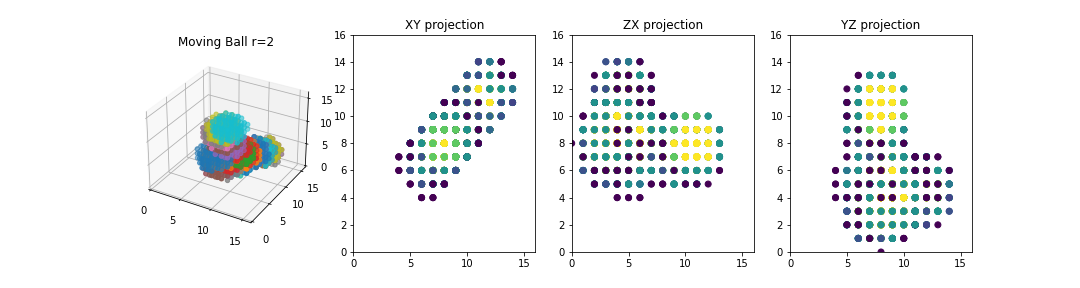
\includegraphics[width=0.95\linewidth]{GPVAE3D/images/result_projection2}}
\end{figure}
\section{Results}
Video samples of length 30 and each frame of size $16X16X16$ generated by GP are fed to the network. These samples were unseen by the network. Using the posterior mean vector from output we predict the ground truth trajectory by linear transformation that minimize the mean square error. The linear transformation is applied to rotate the predicted trajectory to true trajectory. The results (\figureref{fig:result_final2}) shows that predicted trajectories are good reproduction of original. All the code used for this work is present in this repo \url{https://github.com/bdubey/ml_project_gpvae} 

\begin{figure}[!htpb]
\floatconts
  {fig:result_final2}
  {\caption{First Row: Moving ball in a cube of size 16\\
  Second Row: Ground truth(Blue) and the reconstructed trajectory(Orange)}}
    {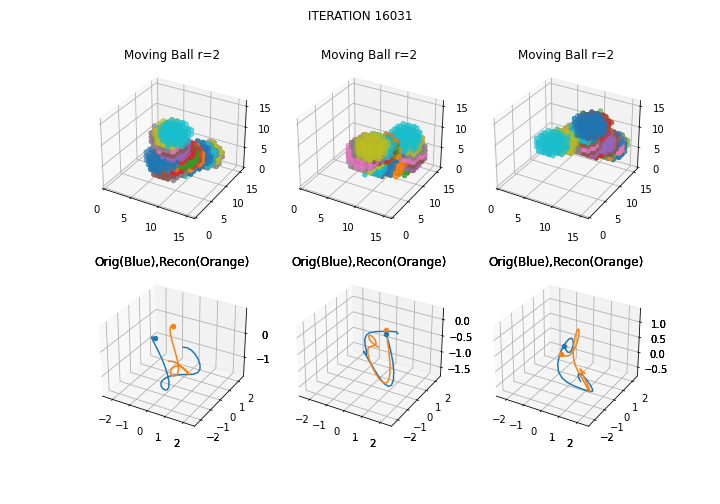
\includegraphics[width=0.95\linewidth]{GPVAE3D/images/result_final2}}
\end{figure}


\acks{}
Thanks Evgenii Egorov for providing mentorship during project.
\bibliography{gpvae3d}
\end{document}
